\documentclass[t]{beamer}
\usepackage{listings}
\usepackage{minted}
\usepackage{graphicx}
\lstset{basicstyle=\ttfamily,
  showstringspaces=false,
  commentstyle=\color{red},
  keywordstyle=\color{blue}
  breaklines=true,
}


\usetheme{CambridgeUS}
\begin{document}

\begin{frame}{Introduction to git}

Why git?
\begin{itemize}
    \item version control
    \item ease of sharing 
    \item organization
    \item backup
    \item facilitate collaboration
\end{itemize}



\end{frame}

\begin{frame}[fragile]
\frametitle{Installing git}
Linux
\begin{enumerate}
    \item Install with package manager
    \begin{minted}[breaklines, linenos]{bash}
    pacman -S git
    \end{minted}
\end{enumerate}

Windows
\begin{enumerate}
    \item Intall "git bash for Windows"
\end{enumerate}
\item Install "git bash for Windows"

MacOS
\begin{enumerate}
    \item Download and Install brew, a package manager for Macs

    \item Install git
    \begin{minted}[breaklines, linenos]{bash}
    brew install git
    \end{minted}
\end{enumerate}

\end{frame}

\begin{frame}[fragile]{Setting up git}

\begin{itemize}
    \item git needs a name and email to associate with it
    \begin{minted}{bash}
    git config --global user.name "John Doe"
    git config --global user.email johndoe@example.com
    \end{minted}
    \vspace*{\fill}
\end{itemize}
\begin{center}
    
\includegraphics[width = .2\textwidth]{gitlogo}
\end{center}

    
\end{frame}

\begin{frame}[fragile]
\frametitle{Basic commands}
\begin{itemize}
    \item init
    Initializes a git repository
    \begin{minted}{bash}
    git init <repo-name>
    \end{minted}
    \item clone
    Copies a git repository from a remote host like Github
    \begin{minted}{bash}
    git clone <URL-of-remote-repo>
    \end{minted}
    \item pull
     Pulls changes from the remote repository
    \begin{minted}{bash}
    git pull
    \end{minted}
   
\end{itemize}

\end{frame}

\begin{frame}[fragile]{Version control commands}
\begin{itemize}
    \item add
    Tells git what files you would like to keep track of for later commits
    \begin{minted}{bash}
    git add <list-of-files>
    \end{minted}
    \item stage
    Stashes any changes you made to the repo since last commit.
    \begin{minted}{bash}
    git stage <list-of-files>
    \end{minted}
    \item commit
    The bread and butter of git; writes changes to the repo
    \begin{minted}{bash}
    git commit -m <comment>
    \end{minted}

\end{itemize}

\end{frame}


\begin{frame}[fragile]{Publishing commands}
\begin{itemize}
    \item push Takes any commits you have and merges them to the remote repo
    \begin{minted}{bash}
    git push <remote-name> <branch-name>
    \end{minted}
    \item tag Marks a commit as special, used for keeping track of specific points in the code
    \begin{minted}{bash}
    git tag -a <tag-name> -m <comment>
    \end{minted}
    \item remote Adds a new remote that you can push to
    \begin{minted}{bash}
    git remote <new-remote-name> <remote-URL>
    \end{minted}
    
\end{itemize}
    
\end{frame}

\begin{frame}[fragile]{Branching}

  \begin{columns}[T]
    \begin{column}{.5\textwidth}
     \begin{block}{}
     \begin{itemize}
         \item Branching allows for multiple versions to exist at once
         \item Example: stable working code, create a new branch to add new features

     \end{itemize}
    \end{block}
    \end{column}
    \begin{column}{.5\textwidth}
    \begin{block}{}
% Your image included here
    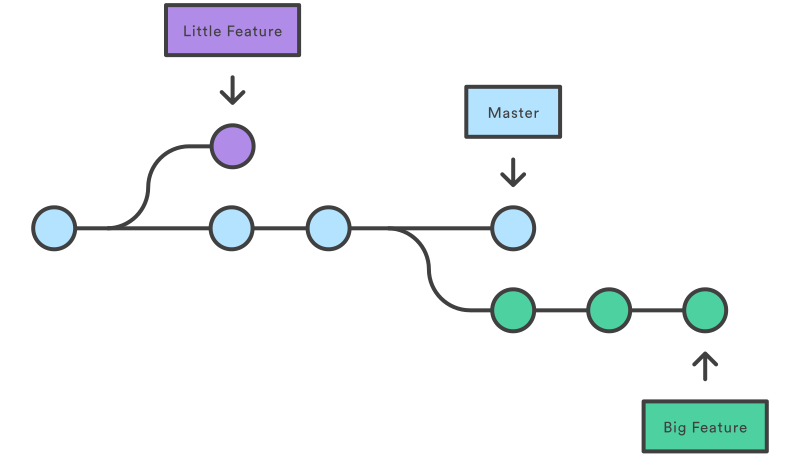
\includegraphics[width = \textwidth]{branches.png}
    \end{block}
    \end{column}
  \end{columns}
 
 \begin{itemize}
          \item command
         \begin{minted}{bash}
        git checkout -b <new-branch>
         \end{minted}
\end{itemize}
    
\end{frame}

\begin{frame}{Automation}
\begin{itemize}
    \item Use git to trigger automation pipelines
    \item For example, a tagging event could trigger Github to compile a specific version of your paper from \LaTeX
\end{itemize}

\end{frame}
    

\begin{frame}{Example paper workflow}
\begin{enumerate}
    \item Start paper on Overleaf
    \item Clone the repo to Github
    \item Add compilation automation triggered from tags
    \item Whenever you want a new pdf to be published, create a tag and push it. 
\end{enumerate}
    
\end{frame}

\end{document}
